\section{Durchführung}
\label{sec:Durchführung}

% Was wurde gemessen bzw. welche Größen wurden variiert?

\begin{figure}
    \centering
    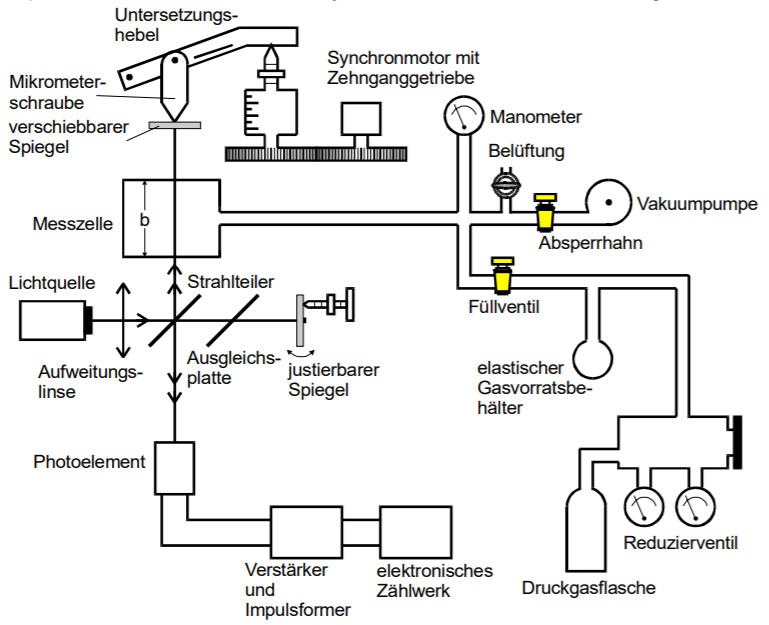
\includegraphics[width=0.4\textwidth]{images/bild4.png}
    \caption{Versuchsaufbau der gesamten Messapperatur.\cite{V401}}
    \label{fig:bild4}
\end{figure}

Zu Beginn der Messung müssen die Spiegel und LASER richtig abgestimmt werden. 
Auf dem Photoelement, also dem Detektor werden die beiden hellsten Reflektionen aus gemacht und übereinander gebracht.
Außerdem wird die Höhe des Photoelements eingestellt, sodass die Strahlen des LASERS auf den Eintrittsspalt treten.
Der justierbare Spiegel wird von einem Motor angetrieben, dieser wird vor der Messung auf eine möglichst genauen Wert eingestellt.
Zudem wird die Hebelübersetzung notiert, die auf dem Gerät angegeben ist. 
Der Motor wird in einer Geschwindigkeit betrieben, in der alle Impulse gezählt werden können. 
Nach etwa 3000 gemessenen Interferenzen wird die Messung gestoppt und der Wert für $d$ wird notiert. 
Diese Messung wird zehn mal durchgeführt.

Für den zweiten Teil der Messung wird die Messzelle auf den Druck $\acute{p}$ evakuiert. 
Dieser Wert wird notiert.
Dann wird der Druck wieder normalisiert, in dieser Zeit werden Interferenzen gezählt.
Der Druck der sich danach einstellt, wird als $p_0$ ebenfalls notiert.
Diese Messung wird fünf mal durchgeführt.